\section{Auswertung}
\label{sec:Auswertung}

\subsection{Bestimmung der Gitterkonstanten $g$}
Die gemessenen Winkel entstehen durch Beugung des Lichtes an einem Reflexionsgitter. Für die weitere Auswertung wird daher die Gitterkonstante $g$ benötigt. Dazu wird das bekannte Spektrum einer Quecksilberdampflampe untersucht. In Tabelle \ref{tab:hgspektrum} sind die Winkel $\tilde{\varphi}$ aufgetragen, unter denen die verschiedenen Spektrallinien auftreten. Zur Bestimmung der tatsächlichen Beugungswinkel müssen einige Korrekturen durchgeführt werden. Alle Winkel sind relativ zur Position des nullten Maximums bei $\varphi_0=323,6\,\si\degree$ gemessen. Daher muss die Differenz $\tilde{\varphi}-\varphi_0=\varphi_\mathup{diff.}$ gebildet werden. 
 Hinzu kommt, dass einlaufender und reflektierter Strahl anders als beim Transmissionsgitter einen Winkel von $2\beta=90\,\si\degree$ einschließen. Für die wirklichen Beugungswinkel $\varphi$ gilt also $\varphi=\varphi_\mathup{diff.}-\beta$.
Dargestellt wird der geometrische Zusammenhang in Abbildung \ref{fig:winkelbeziehungen}.

\begin{figure}
	\centering
	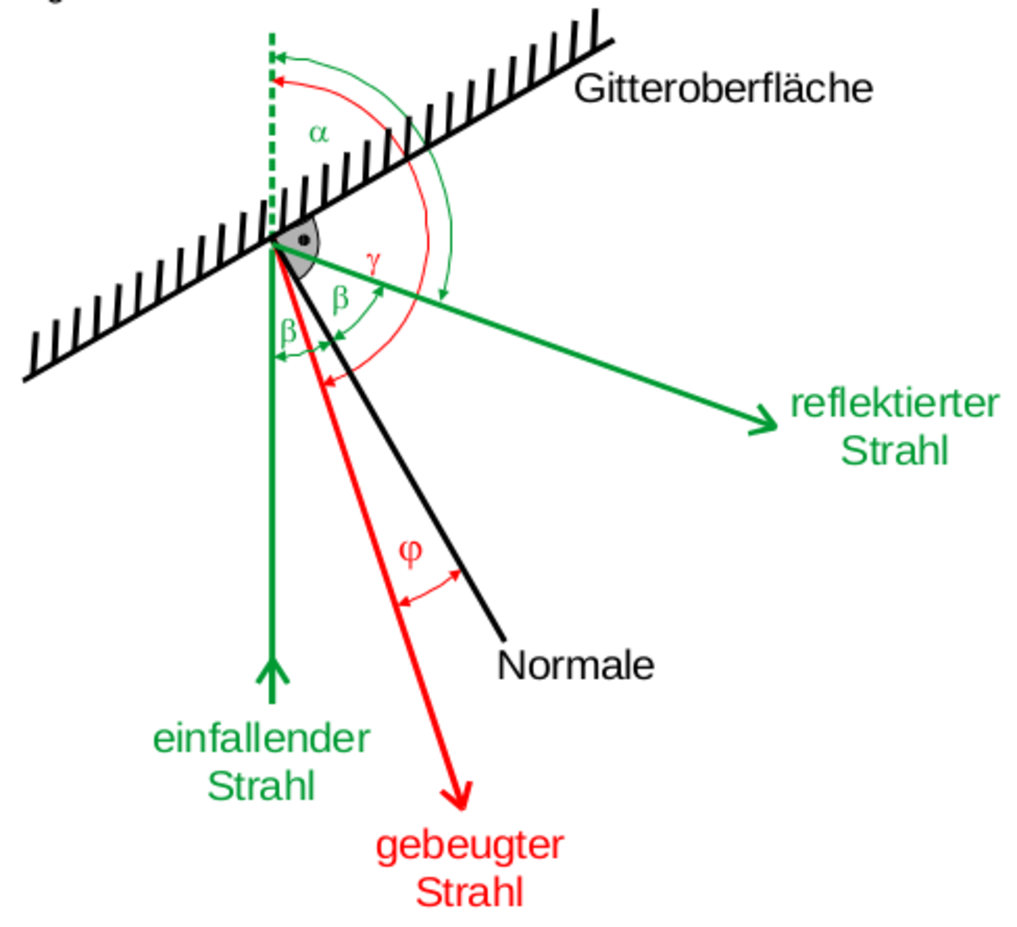
\includegraphics[width=0.5\textwidth]{Bilder/Winkelbeziehungen.pdf}
	\caption{Winkelbeziehungen bei Verwendung eines Reflexionsgitters.}%\cite{skript}
	\label{fig:winkelbeziehungen}
\end{figure}

Um die Gitterkonstante $g$ zu bestimmen wird $\sin{\beta}+\sin{\varphi}$ in Abhängigkeit von der Wellenlänge $\lambda$ aufgetragen. Die Formel kann abgeleitet werden aus Abbildung \ref{fig:winkelbeziehungen}. Es gilt
\begin{equation}
\sin{\beta}+\sin{\varphi}=\frac{\lambda}{g}.
\end{equation}
Daraus ergibt sich mit linearer Regression eine Geradengleichung
\begin{equation}
f(x)= \underbrace{(0.001192 \pm 0.000006)\,\frac{1}{\si{\nano\meter}}}_{Steigung\,\triangleq\,\sfrac{1}{g}}x-(0.002 \pm 0.003)
\label{eq:lin_reg}
\end{equation}
deren reziproke Steigung dem Wert der Gitterkonstanten
\begin{equation}
g=(839 \pm 3)\,\si{\nano\meter}
\label{eq:gitterkonst}
\end{equation}
entspricht.

\begin{figure}
	\centering
	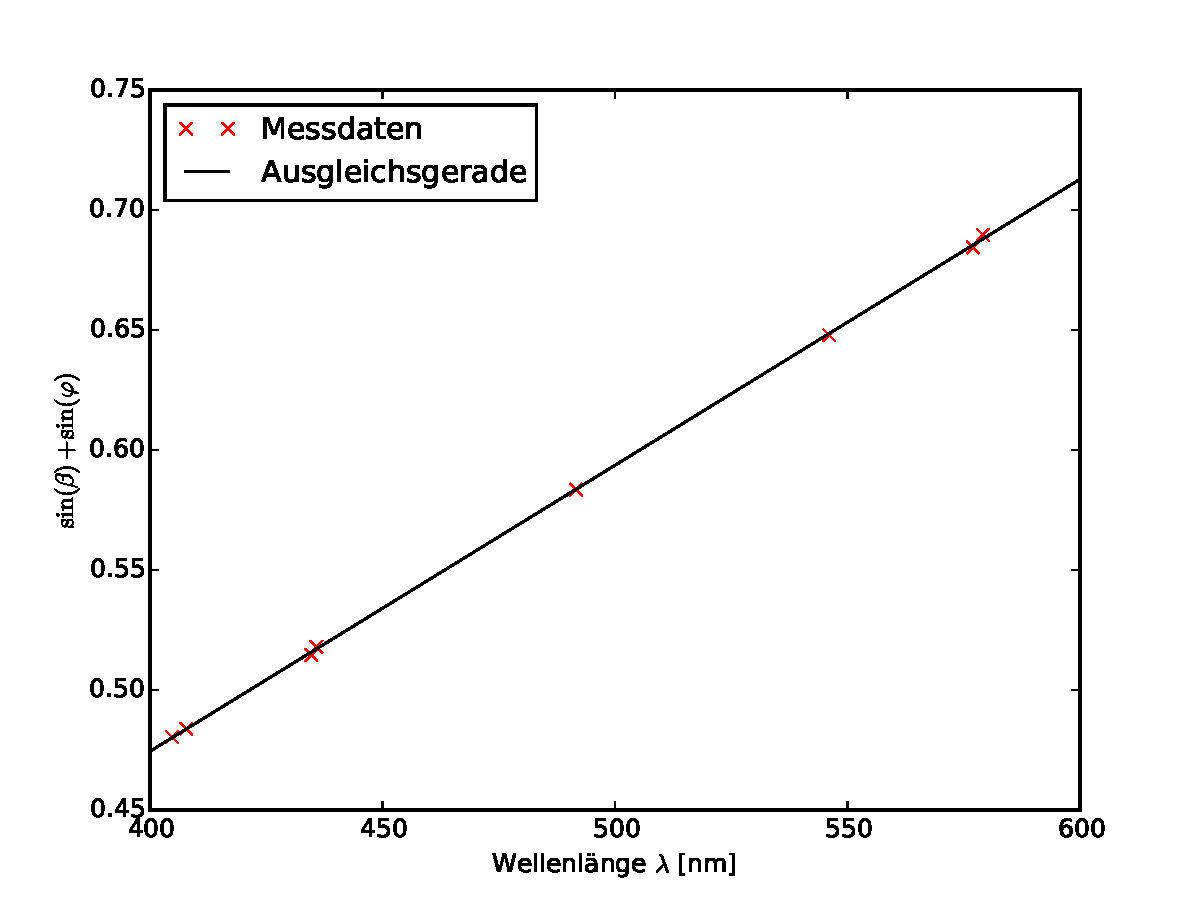
\includegraphics[width=\textwidth]{Bilder/Gitterkonstante.pdf}
	\caption{Lineare Regression zur Bestimmung von $g$.}
	\label{fig:lin_reg}
\end{figure}


\subsection{Untersuchung der Alkalispektren}

Es werden die Spektren einer Natrium-\footnote{\Bat}, Kalium - und Rubidiumdampflampe ausgemessen. Nähere erfahren die Dublett-Linien. Die beobachteten Linien entstehen durch aufspalten des 3P-Niveaus (Na), 4P-Niveaus (Ka) und 5P-Niveaus (Rb).  Da sie sehr nahe beieinanderliegen wird zur Abstandsmessung ein Okularmikrometer benutzt. Dieses wird zuvor geeicht, wobei $143$ Skalenteile einer Winkeländerung von $\SI{0,3}{\degree}$ entsprechen. Damit kann der Eichfaktor zu $\gamma=0.015\,\si{\nano\meter}\,/\text{Skt.}$ berechnet werden. 
In Tabelle \ref{tab:spektren} werden die aufgenommenen, sowie um $\varphi_0$ und $\beta$ korrigierten Wete gelistet. Der Winkel $\varphi$, unter welchem die Liniendubletts zu sehen sind, wird durch Mittelwertsbildung der Winkel beider Linien ermittelt. Zwischen den Linien liegt eine Entfernung $\Delta{s}$ . Die Wellenlänge $\lambda$, sowie der Wellenlängenunterschied $\Delta{\lambda}$ werden nach THEORIE berechnet. Mit Gleichung BÖLAA kann nun die Energiedifferenz $\Delta{E}$ und damit die Abschirmungszahl $\sigma$ bestimmt werden.
Die Abschirmungszahlen ergeben sich mit den Werten aus Tabelle \ref{tab:spektren} zu 
\begin{align}
\sigma_\mathup{Na}&=\SI{8.424285(3)}{} \\
\sigma_\mathup{K\:}&=\SI{12.988059(5)}{}\\
\sigma_\mathup{Rb}&=\SI{26.8692(2)}{}.
\end{align}
